\newpage
\section{Homotecia}



\subsection{Homotecia en polígonos}

\begin{section-definition.tcb}{Homotecia}{homothety-definition}
    La homotecia es una transformación geométrica la que, dado un punto $P$ en el plano y un número real $k \neq 0$, traslada cada punto $Q$ del plano a un punto $Q'$ de modo que
    \begin{itemize}
        \item Los punto $P$, $Q$ y $Q'$ son colineaes, y
        \item $\dfrac{Q' P}{QP} = k$.
    \end{itemize}
\end{section-definition.tcb}

El punto $P$ se llama \textbf{centro de homotecia}, $k$ es la \textbf{razón de homotecia} y los punto $Q$ y $Q'$ son nombrados \textbf{elementos homólogos}.

Si $k$ es un número real positivo, diremos que la homotecia es \textbf{directa}; en este caso, los elementos homólogos yacen a un mismo lado del centro de homotecia $P$; en contraste, la homotecia es \textbf{inversa} si $k$ es negativo, en la que los elementos homólogos yacen en lados opuestos con respecto a $P$.

En caso de aplicar una homotecia con centro $P$ y razón $k$ a $n$ puntos $P_1$, $P_2$, $\cdots$, $P_n$ y obtener los puntos homólogos $P'_1$, $P'_2$, $\cdots$, $P'_n$, se dice que los polígonos, no necesariamente convexos, $P_1 P_2 \cdots P_n$ y $P'_1 P'_2 \cdots P'_n$ son \textbf{homotéticos}.
En esta situación todos los elementos correspondientes (tales como lados, diagonales, etc) también son elementos homólgos.

\begin{figure}[H]
    \centering
    \begin{tikzpicture}[xscale = 1.5, yscale = 1.5]

\end{tikzpicture}
    \caption{Una homotecia directa envía \theTriangle{ABC} a \theTriangle{A' B' C'} y una inversa manda \theTriangle{ABC} a \theTriangle{A'' B'' C''}.}
    \label{fig:homothety-definition}
\end{figure}

\begin{remark.tcb}
    Para una mayor fomalidad, usaremos la siguiente notación;
    \[
        \homothety{O}{\pm k}{P}{P'}
    \]
    La cual se lee ``La homotecia directa/inversa con centro $O$ y razón $k$, envía $P$ a $P'$."
\end{remark.tcb}

Utilizando la notación, para describir la figura~\ref{fig:homothety-definition}, quedaría como:
\[
    \homothety{P}{k_1}{\theTriangle{ABC}}{\theTriangle{A' B' C'}} \quad \text{ y } \quad \homothety{P}{- k_2}{\theTriangle{ABC}}{\theTriangle{A'' B'' C''}}.
\]

\subsubsection{Propiedades}
Entre las propiedades más importantes de la homotecia tenemos:
\begin{itemize}
    \item Los lados correspondientes de dos figuras homotéticas son paralelos.
    \item La razón de las áreas de dos figuras homotéticas es igual al cuadrado de la razón de homotecia.
    \item Los puntos notables de figuras homotéticas son siempre colineales con el centro de homotecia.
    \item La homotecia perserva ángulo y por ende tangencias.
\end{itemize}


\subsubsection{Ejemplos}

\begin{section-example.tcb}{La recta de Euler}{}
    Dado un triángulo cualquiera el circuncentro, ortocentro y baricentro son colineales.
\end{section-example.tcb}

\begin{multicols}{2}

    \begin{solution}
        Sea \theTriangle{ABC} el triángulo, $H$ y $O$ su ortocentro y circuncentro; $D$ y $E$ pies de alturas desde $A$ y $B$; $L$ y $M$ puntos medios de $BC$ y $AC$, respectivamente.

        Claramente \homothety{G}{-2}{\theTriangle{LMO}}{\theTriangle{ABH}}, es decir los triángulos \theTriangle{ABH} y \theTriangle{LMO} son homotéticos, pues sus lados son paralelos y
        \[
            k = \dfrac{AB}{LM} = -2.
        \]
        Luego, $AL$, $BM$ y $HO$ son concurrentes en el baricentro $G$.
    \end{solution}

    \begin{figure}[H]
        \centering
        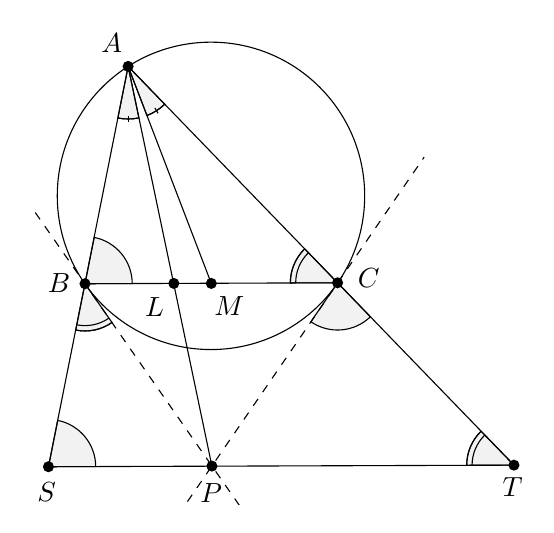
\begin{tikzpicture}[scale = 0.4]
    \clip(-2.36,-10.08) rectangle (13.47,5.06);
    \draw [shift={(-0.54,-3.07)},fill=black,fill opacity=0.05] (0,0) -- (0.2:1.5) arc (0.2:78.71:1.5) -- cycle;
    \draw [shift={(7.48,-3.04)},fill=black,fill opacity=0.05] (0,0) -- (-124.46:1.5) arc (-124.46:-45.95:1.5) -- cycle;
    \draw [shift={(-1.7,-8.88)},fill=black,fill opacity=0.05] (0,0) -- (0.2:1.5) arc (0.2:78.71:1.5) -- cycle;
    \draw [shift={(-0.54,-3.07)},fill=black,fill opacity=0.05] (0,0) -- (-101.29:1.5) arc (-101.29:-55.14:1.5) -- cycle;
    \draw [shift={(7.48,-3.04)},fill=black,fill opacity=0.05] (0,0) -- (134.05:1.5) arc (134.05:180.2:1.5) -- cycle;
    \draw [shift={(13.08,-8.83)},fill=black,fill opacity=0.05] (0,0) -- (134.05:1.5) arc (134.05:180.2:1.5) -- cycle;
    \draw [shift={(0.83,3.83)},fill=black,fill opacity=0.05] (0,0) -- (-101.29:1.67) arc (-101.29:-78.18:1.67) -- cycle;
    \draw [shift={(0.83,3.83)},fill=black,fill opacity=0.05] (0,0) -- (-69.06:1.67) arc (-69.06:-45.95:1.67) -- cycle;
    \draw(3.46,-0.28) circle (4.88cm);
    \draw (-0.54,-3.07)-- (7.48,-3.04);
    \draw (0.83,3.83)-- (-1.7,-8.88);
    \draw (0.83,3.83)-- (13.08,-8.83);
    \draw (-1.7,-8.88)-- (13.08,-8.83);
    \draw (0.83,3.83)-- (3.49,-8.86);
    \draw (0.83,3.83)-- (3.47,-3.06);
    \draw [dash pattern=on 3pt off 3pt,domain=-2.1176316762214267:13.472829432059696] plot(\x,{(-21.59-8.05*\x)/5.61});
    \draw [dash pattern=on 3pt off 3pt,domain=-2.361745286484902:10.226227746616733] plot(\x,{(--93.93-9.81*\x)/-6.74});
    \draw [shift={(-0.54,-3.07)}] (-101.29:1.5) arc (-101.29:-55.14:1.5);
    \draw [shift={(-0.54,-3.07)}] (-101.29:1.33) arc (-101.29:-55.14:1.33);
    \draw [shift={(7.48,-3.04)}] (134.05:1.5) arc (134.05:180.2:1.5);
    \draw [shift={(7.48,-3.04)}] (134.05:1.33) arc (134.05:180.2:1.33);
    \draw [shift={(13.08,-8.83)}] (134.05:1.5) arc (134.05:180.2:1.5);
    \draw [shift={(13.08,-8.83)}] (134.05:1.33) arc (134.05:180.2:1.33);
    \draw [shift={(0.83,3.83)}] (-101.29:1.67) arc (-101.29:-78.18:1.67);
    \draw(0.84,2.27) -- (0.84,2.07);
    \draw [shift={(0.83,3.83)}] (-69.06:1.67) arc (-69.06:-45.95:1.67);
    \draw(1.68,2.51) -- (1.78,2.34);
    \begin{scriptsize}
        \normalsize
        \fill [color=black] (0.83,3.83) circle (5pt);
        \draw[color=black] (0.31,4.56) node {$A$};
        \fill [color=black] (3.49,-8.86) circle (5pt);
        \draw[color=black] (3.47,-9.7) node {$P$};
        \fill [color=black] (-0.54,-3.07) circle (5pt);
        \draw[color=black] (-1.36,-3.04) node {$B$};
        \fill [color=black] (7.48,-3.04) circle (5pt);
        \draw[color=black] (8.47,-2.88) node {$C$};
        \fill [color=black] (-1.7,-8.88) circle (5pt);
        \draw[color=black] (-1.76,-9.68) node {$S$};
        \fill [color=black] (13.08,-8.83) circle (5pt);
        \draw[color=black] (13.04,-9.54) node {$T$};
        \fill [color=black] (2.28,-3.06) circle (5pt);
        \draw[color=black] (1.67,-3.81) node {$L$};
        \fill [color=black] (3.47,-3.06) circle (5pt);
        \draw[color=black] (4.04,-3.78) node {$M$};
    \end{scriptsize}
\end{tikzpicture}
        \caption{La Lecta de Euler.}
    \end{figure}
\end{multicols}


\begin{section-example.tcb}{La circunferencia de los nueve puntos}{}
    Dado un triángulo cualquiera, los pies de las alturas, los puntos medios de los lados, y los puntos medios de los segmentos que van del vértice al ortocentro están en una misma circunferencia.
\end{section-example.tcb}
\begin{solution}
    \begin{multicols}{2}
        Sea \theTriangle{ABC} el triángulo, $D$, $E$ y $F$ pies de alturas, $X$, $Y$ y $Z$ intersecciones de las alturas con el circuncírculo, $L$, $M$ y $N$ puntos medios, $A'$, $B'$ y $C$ puntos diametralmente opuestos, y $P$, $Q$ y $R$ puntos medios de $AH$, $BH$ y $CH$, respectivamente.
        El centro de esta circunferencia se ubica sobre la recta que va del ortocentro al circuncentro.


        Recordemos que $D$, $E$ y $F$ son puntos medios de $HX$, $HY$ y $HX$, respectivamente.
        Y también que $L$, $M$ y $N$ son puntos medios de $HA'$, $HB'$ y $HC'$, respectivamente.


        De este modo el eneágono $AC' ZBXA' CB' Y$ es homotético a $PNFQDLRME$ con razón $1/2$ y centro $H$, y como el primero es cíclico, el segundo también debe serlo.

        Pero como el centro de homotecia es $H$ y la razón \inverseOfD{2}, el centro del círculo de los nueve puntos debe ser el punto medio de $OH$.\qedhere
        \begin{figure}[H]
            \centering
            \definecolor{qqwwcc}{rgb}{0,0.4,0.8}

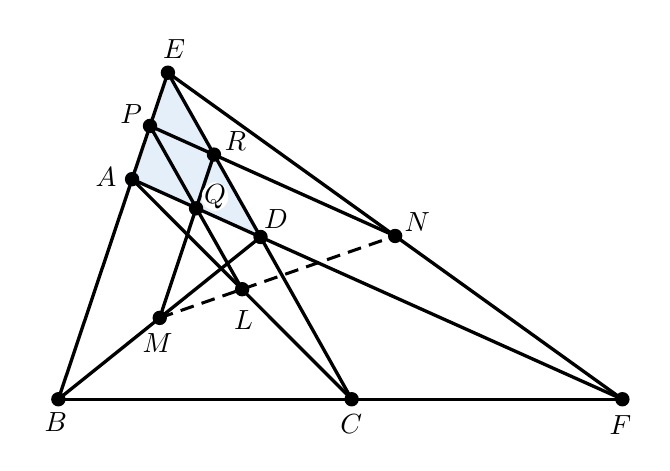
\begin{tikzpicture}[scale = 0.65]
    \clip(-1.86,-1.14) rectangle (10.13,6.98);
    \fill[line width=0pt,color=qqwwcc,fill=qqwwcc,fill opacity=0.1] (0.88,6.1) -- (0.18,4.02) -- (2.69,2.89) -- cycle;
    \draw [line width=1.2pt] (-1.26,-0.28)-- (0.18,4.02);
    \draw [line width=1.2pt] (4.47,-0.28)-- (2.69,2.89);
    \draw [line width=1.2pt] (2.69,2.89)-- (0.18,4.02);
    \draw [line width=1.2pt] (-1.26,-0.28)-- (9.76,-0.28);
    \draw [line width=1.2pt] (2.69,2.89)-- (9.76,-0.28);
    \draw [line width=1.2pt] (2.69,2.89)-- (0.88,6.1);
    \draw [line width=1.2pt] (0.18,4.02)-- (0.88,6.1);
    \draw [line width=1.2pt] (0.88,6.1)-- (9.76,-0.28);
    \draw [line width=1.2pt] (-1.26,-0.28)-- (2.69,2.89);
    \draw [line width=1.2pt] (0.18,4.02)-- (4.47,-0.28);
    \draw [line width=1.2pt] (0.53,5.06)-- (2.33,1.87);
    \draw [line width=1.2pt] (1.78,4.5)-- (0.72,1.31);
    \draw [line width=1.2pt] (0.53,5.06)-- (5.32,2.91);
    \draw [line width=1.1pt,dash pattern=on 5pt off 3pt] (0.72,1.31)-- (5.32,2.91);
    \begin{scriptsize}
        \normalsize
        \fill [color=black] (0.18,4.02) circle (4.0pt);
        \draw[color=black] (-0.33,4.06) node {$A$};
        \fill [color=black] (-1.26,-0.28) circle (4.0pt);
        \draw[color=black] (-1.31,-0.73) node {$B$};
        \fill [color=black] (4.47,-0.28) circle (4.0pt);
        \draw[color=black] (4.46,-0.76) node {$C$};
        \fill [color=black] (2.69,2.89) circle (4.0pt);
        \draw[color=black] (2.99,3.25) node {$D$};
        \fill [color=black] (0.88,6.1) circle (4.0pt);
        \draw[color=black] (1,6.57) node {$E$};
        \fill [color=black] (9.76,-0.28) circle (4.0pt);
        \draw[color=black] (9.72,-0.78) node {$F$};
        \fill [color=black] (0.72,1.31) circle (4.0pt);
        \draw[color=black] (0.68,0.82) node {$M$};
        \fill [color=black] (2.33,1.87) circle (4.0pt);
        \draw[color=black] (2.36,1.26) node {$L$};
        \fill [color=black] (1.43,3.45) circle (4.0pt);
        \draw[color=black] (1.8,3.68) node[fill = white, rounded corners = 5pt, inner sep=0.8pt] {$Q$};
        \fill [color=black] (0.53,5.06) circle (4.0pt);
        \draw[color=black] (0.16,5.29) node {$P$};
        \fill [color=black] (1.78,4.5) circle (4.0pt);
        \draw[color=black] (2.2,4.77) node[fill = white, rounded corners = 5pt, inner sep=0.8pt] {$R$};
        \fill [color=black] (5.32,2.91) circle (4.0pt);
        \draw[color=black] (5.75,3.19) node {$N$};
    \end{scriptsize}
\end{tikzpicture}
            \caption{Circunferencia de los nueve puntos.}
        \end{figure}
    \end{multicols}
\end{solution}



\subsection{Homotecia en circunferencias}
Dadas dos circunferencias de radios finitos y no concéntricas, siempre existen dos homotecias que transforman una circunferencia en la otra.

\begin{section-definition.tcb}{Exsimilicentro e insimilicentro}{}
    Sean dos circunferencias $\Omega_1$ y $\Omega_2$ con centros $O_1$ y $O_2$ y radios $r_1$ y $r_2$, respectivamente.
    Consideremos los puntos $P$ y $Q$ tales que
    \[
        \homothety{P}{\dfrac{r_1}{r_2}}{\Omega_1}{\Omega_2} \quad \  \text{y}\  \quad \homothety{Q}{-\dfrac{r_1}{r_2}}{\Omega_1}{\Omega_2}.
    \]
    Entonces $P$ y $Q$ son el \textbf{exsimilicentro} e \textbf{insimilicentro} de $\Omega_1$ y $\Omega_2$, respectivamente.
    Además, son puntos únicos.
\end{section-definition.tcb}

¿Cómo construir el exsimilicentro y el insimilicentro?
Un método general es el siguiente: Trazamos dos diámetros $AB$ y $CD$ en $\Omega_1$ y $\Omega_2$, respectivamente, tales que $AB || CD$.
Luego, $P = AD \cap BD$ y $Q = AD \cap BD$.

\begin{figure}[H]
    \centering
    \begin{subfigure}{0.4\textwidth}
    \centering
    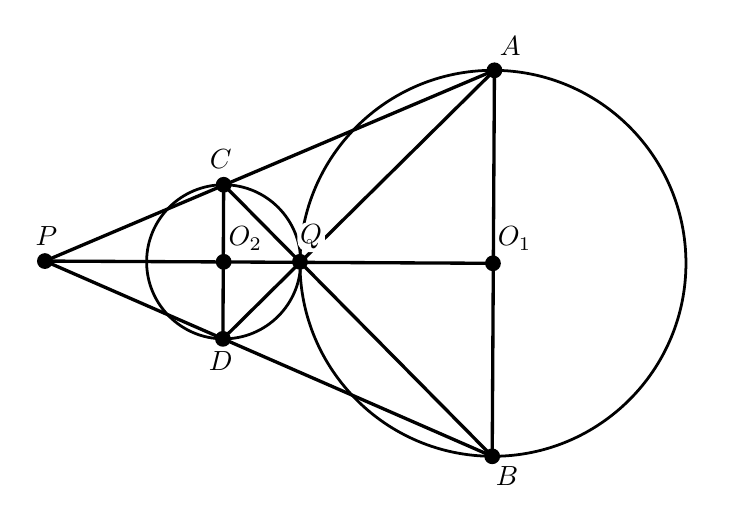
\begin{tikzpicture}[scale = 0.95]
        \clip(3.93,-4.43) rectangle (12.98,1.92);
        \draw [line width=1pt] (10.15,-1.23) circle (2.58cm);
        \draw [line width=1.2pt] (10.17,1.35)-- (10.14,-3.81);
        \draw [line width=1pt](6.55,-1.21) circle (1.03cm);
        \draw [line width=1.2pt] (10.17,1.35)-- (6.54,-2.24);
        \draw [line width=1.2pt] (10.14,-3.81)-- (6.55,-0.18);
        \draw [line width=1.2pt] (4.16,-1.2)-- (10.17,1.35);
        \draw [line width=1.2pt] (4.16,-1.2)-- (10.14,-3.81);
        \draw [line width=1.2pt] (6.55,-0.18)-- (6.54,-2.24);
        \draw [line width=1.2pt] (4.16,-1.2)-- (10.15,-1.23);
        \begin{scriptsize}
            \normalsize
            \fill [color=black] (10.15,-1.23) circle (3pt);
            \draw[color=black] (10.44,-0.9) node {$O_1$};
            \fill [color=black] (10.17,1.35) circle (3pt);
            \draw[color=black] (10.38,1.67) node {$A$};
            \fill [color=black] (10.14,-3.81) circle (3pt);
            \draw[color=black] (10.34,-4.07) node {$B$};
            \fill [color=black] (7.57,-1.21) circle (3pt);
            \draw[color=black] (7.72,-0.88) node[fill = white, rounded corners = 4pt, inner sep=1pt] {$Q$};
            \fill [color=black] (6.55,-1.21) circle (3pt);
            \draw[color=black] (6.84,-0.9) node {$O_2$};
            \fill [color=black] (6.55,-0.18) circle (3pt);
            \draw[color=black] (6.51,0.16) node {$C$};
            \fill [color=black] (6.54,-2.24) circle (3pt);
            \draw[color=black] (6.51,-2.54) node {$D$};
            \fill [color=black] (4.16,-1.2) circle (3pt);
            \draw[color=black] (4.18,-0.86) node {$P$};
        \end{scriptsize}
    \end{tikzpicture}
\end{subfigure}
\hspace{0.1\textwidth}
\begin{subfigure}{0.4\textwidth}
    \centering
    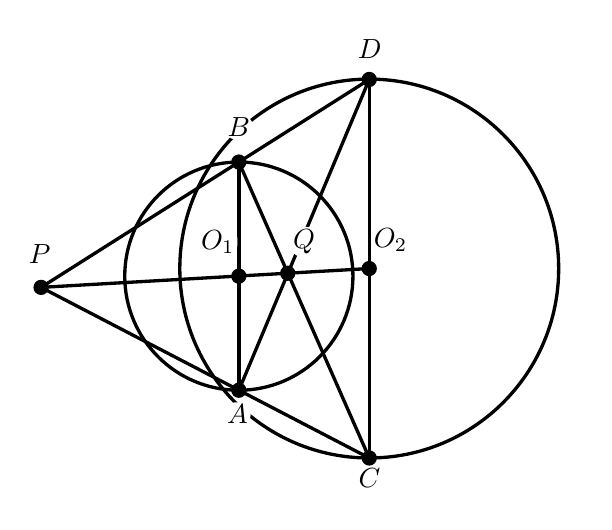
\begin{tikzpicture}[scale = 0.46]
        \clip(-0.43,-0.99) rectangle (14.92,12.11);
        \draw [line width=1.2pt] (5.4,5.25) circle (3.15cm);
        \draw [line width=1.2pt] (9,5.46) circle (5.23cm);
        \draw [line width=1.2pt] (-0.06,4.94)-- (9,0.23);
        \draw [line width=1.2pt] (-0.06,4.94)-- (9,10.68);
        \draw [line width=1.2pt] (-0.06,4.94)-- (9,5.46);
        \draw [line width=1.2pt] (5.4,2.1)-- (5.4,8.4);
        \draw [line width=1.2pt] (9,0.23)-- (9,10.68);
        \draw [line width=1.2pt] (5.4,2.1)-- (9,10.68);
        \draw [line width=1.2pt] (9,0.23)-- (5.4,8.4);
        \begin{scriptsize}
            \normalsize
            \fill [color=black] (5.4,5.25) circle (6pt);
            \draw[color=black] (4.82,6.2) node[fill = white, rounded corners = 4pt, inner sep=1pt] {$O_1$};
            \fill [color=black] (5.4,2.1) circle (6pt);
            \draw[color=black] (5.36,1.43) node[fill = white, rounded corners = 4pt, inner sep=1pt] {$A$};
            \fill [color=black] (5.4,8.4) circle (6pt);
            \draw[color=black] (5.4,9.36) node[fill = white, rounded corners = 4pt, inner sep=1pt] {$B$};
            \fill [color=black] (9,0.23) circle (6pt);
            \draw[color=black] (9.01,-0.33) node[fill = white, rounded corners = 4pt, inner sep=1pt] {$C$};
            \fill [color=black] (9,5.46) circle (6pt);
            \draw[color=black] (9.59,6.24) node[fill = white, rounded corners = 4pt, inner sep=1pt] {$O_2$};
            \fill [color=black] (9,10.68) circle (6pt);
            \draw[color=black] (9.01,11.53) node[fill = white, rounded corners = 4pt, inner sep=1pt] {$D$};
            \fill [color=black] (6.75,5.33) circle (6pt);
            \draw[color=black] (7.2,6.2) node[fill = white, rounded corners = 4pt, inner sep=1pt] {$Q$};
            \fill [color=black] (-0.06,4.94) circle (6pt);
            \draw[color=black] (-0.1,5.87) node[fill = white, rounded corners = 4pt, inner sep=1pt] {$P$};
        \end{scriptsize}
    \end{tikzpicture}
\end{subfigure}
    \caption{Trazado general del exsimilicentro e insimilicentro de dos circunferencias.}
\end{figure}

Una situación particular y muy frecuente en competiciones matemáticas sucede cuando $\Omega_1$ y $\Omega_2$ están en ``posición general", es decir, no son cocéntricas, sus radios poseen distinta longitud positiva y no poseen puntos comunes.
En este contexto, podemos obtener el exsimilicentro $P$ como el punto común de las tangentes externas de $\Omega_1$ y $\Omega_2$, mientras tanto, $Q$ sería el punto de intersección de las tangentes internas de $\Omega_1$ y $\Omega_2$, de aquí los prefijos ex- e in-, como se muestra en la figura~\ref{fig:ex-in-similaricenter}.

\begin{figure}[H]
    \centering
    \definecolor{qqqqcc}{rgb}{0,0,0.8}
\definecolor{qqqqzz}{rgb}{0,0,0.6}
\definecolor{ccqqqq}{rgb}{0.8,0,0}
\definecolor{wwwwww}{rgb}{0.4,0.4,0.4}

\begin{subfigure}{0.4\textwidth}
    \centering
    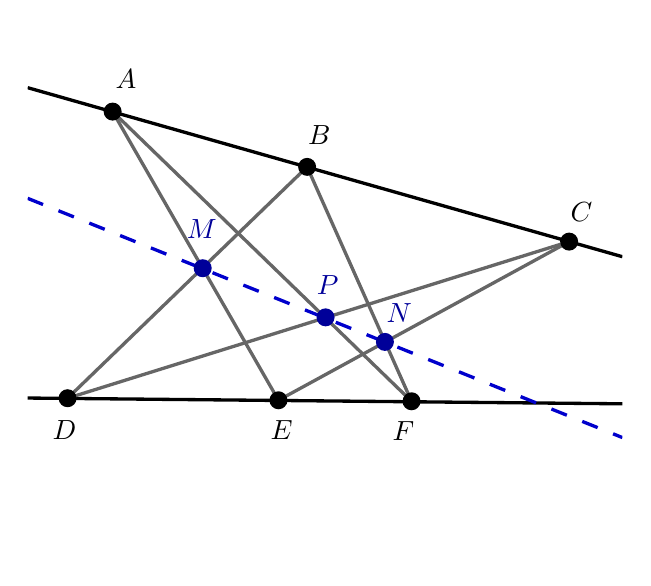
\begin{tikzpicture}[scale = 1.3]
        \clip(-3.03,0.22) rectangle (2.78,5.4);
        \draw [line width=1.2pt,domain=-3.03:2.78] plot(\x,{(--7.51-0.54*\x)/1.9});
        \draw [line width=1.2pt,domain=-3.03:2.78] plot(\x,{(--3.61-0.02*\x)/2.06});
        \draw [line width=1.2pt,color=wwwwww] (-2.2,4.58)-- (-0.58,1.76);
        \draw [line width=1.2pt,color=wwwwww] (-2.2,4.58)-- (0.72,1.75);
        \draw [line width=1.2pt,color=wwwwww] (-2.64,1.78)-- (-0.3,4.04);
        \draw [line width=1.2pt,color=wwwwww] (-2.64,1.78)-- (2.26,3.31);
        \draw [line width=1.2pt,color=wwwwww] (-0.58,1.76)-- (2.26,3.31);
        \draw [line width=1.2pt,color=wwwwww] (-0.3,4.04)-- (0.72,1.75);
        \draw [line width=1.2pt,dash pattern=on 6pt off 6pt,color=qqqqcc,domain=-3.03:2.78] plot(\x,{(--4.5-0.72*\x)/1.79});
        \begin{scriptsize}
            \normalsize
            \fill [color=black] (-2.2,4.58) circle (2.5pt);
            \draw[color=black] (-2.07,4.9) node {$A$};
            \fill [color=black] (-0.3,4.04) circle (2.5pt);
            \draw[color=black] (-0.18,4.35) node {$B$};
            \fill [color=black] (2.26,3.31) circle (2.5pt);
            \draw[color=black] (2.38,3.6) node {$C$};
            \fill [color=black] (-2.64,1.78) circle (2.5pt);
            \draw[color=black] (-2.67,1.47) node {$D$};
            \fill [color=black] (-0.58,1.76) circle (2.5pt);
            \draw[color=black] (-0.55,1.47) node {$E$};
            \fill [color=black] (0.72,1.75) circle (2.5pt);
            \draw[color=black] (0.64,1.46) node {$F$};
            \fill [color=qqqqzz] (-1.32,3.05) circle (2.5pt);
            \draw[color=qqqqzz] (-1.33,3.43) node {$M$};
            \fill [color=qqqqzz] (-0.12,2.57) circle (2.5pt);
            \draw[color=qqqqzz] (-0.1,2.89) node {$P$};
            \fill [color=qqqqzz] (0.46,2.33) circle (2.5pt);
            \draw[color=qqqqzz] (0.6,2.61) node {$N$};
        \end{scriptsize}
    \end{tikzpicture}
    \caption{Transversal $M-P-N$.}
\end{subfigure}
\hspace{0.1\textwidth}
\begin{subfigure}{0.4\textwidth}
    \centering
    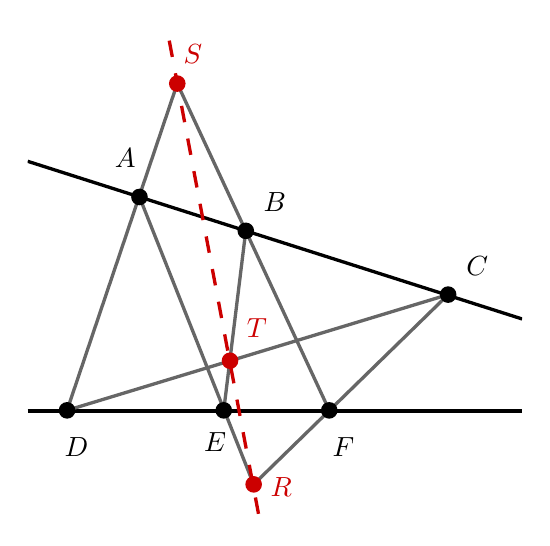
\begin{tikzpicture}[scale = 1]
        \clip(-3.01,-7.4) rectangle (3.27,-1.18);
        \draw [line width=1.2pt,domain=-3.01:3.27] plot(\x,{(-15.04-1.25*\x)/3.92});
        \draw [line width=1.2pt,domain=-3.01:3.27] plot(\x,{(-20.14-0*\x)/3.33});
        \draw [line width=1.2pt,color=wwwwww] (-1.11,-1.89)-- (-2.51,-6.04);
        \draw [line width=1.2pt,color=wwwwww] (-1.11,-1.89)-- (0.82,-6.04);
        \draw [line width=1.2pt,color=wwwwww] (-0.14,-6.98)-- (-1.59,-3.33);
        \draw [line width=1.2pt,color=wwwwww] (2.33,-4.57)-- (-0.14,-6.98);
        \draw [line width=1.2pt,color=wwwwww] (-0.52,-6.04)-- (-0.24,-3.76);
        \draw [line width=1.2pt,color=wwwwww] (-2.51,-6.04)-- (2.33,-4.57);
        \draw [line width=1.2pt,dash pattern=on 6pt off 6pt,color=ccqqqq,domain=-3.01:3.27] plot(\x,{(-7.46-5.09*\x)/0.96});
        \begin{scriptsize}
            \normalsize
            \fill [color=black] (-1.59,-3.33) circle (3pt);
            \draw[color=black] (-1.77,-2.83) node {$A$};
            \fill [color=black] (-0.24,-3.76) circle (3.0pt);
            \draw[color=black] (0.13,-3.4) node {$B$};
            \fill [color=black] (2.33,-4.57) circle (3.0pt);
            \draw[color=black] (2.7,-4.21) node {$C$};
            \fill [color=black] (-2.51,-6.04) circle (3.0pt);
            \draw[color=black] (-2.39,-6.51) node {$D$};
            \fill [color=black] (-0.52,-6.04) circle (3.0pt);
            \draw[color=black] (-0.63,-6.44) node {$E$};
            \fill [color=black] (0.82,-6.04) circle (3.0pt);
            \draw[color=black] (1,-6.51) node {$F$};
            \fill [color=ccqqqq] (-1.11,-1.89) circle (3.0pt);
            \draw[color=ccqqqq] (-0.91,-1.52) node {$S$};
            \fill [color=ccqqqq] (-0.14,-6.98) circle (3.0pt);
            \draw[color=ccqqqq] (0.21,-7.01) node {$R$};
            \fill [color=ccqqqq] (-0.44,-5.41) circle (3.0pt);
            \draw[color=ccqqqq] (-0.1,-5) node {$T$};
        \end{scriptsize}
    \end{tikzpicture}
    \caption{Transversal $S-T-R$.}
\end{subfigure}
    \caption{El exsimilicentro $P$ e insimilicentro $Q$ de $\Omega_1$ y $\Omega_2$.}
    \label{fig:ex-in-similaricenter}
\end{figure}

\begin{section-theorem.tcb}{Monge}{monge-theorem}
    Sean $\Omega_1$, $\Omega_2$ y $\Omega_3$ tres circunferencias.
    Los exsimilicentros $P_1$ de $\Omega_1$ y $\Omega_2$; $P_2$ de $\Omega_2$ y $\Omega_3$, y $P_3$ de $\Omega_3$ y $\Omega_1$ son colineales.
\end{section-theorem.tcb}

\begin{proof}
    Sea $O_1$ el circuncentro de $\Omega_1$ y $r_1$ el radio.
    Se definen de manera análoga $O_2$, $O_3$, $r_2$ y $r_3$.

    Por el teorema de Menelao aplicado al \theTriangle{O_1 O_2 O_3}, es suficiente probar que
    \[
        \ratioCM{O_3}{O_1}{O_2}{P_3}{P_1}{P_2} = 1,
    \]
    \begin{figure}[H]
        \centering
        \definecolor{ttttff}{rgb}{0.2,0.2,1}
%dash pattern=on 5pt off 2pt
%[fill = white, rounded corners = 4pt, inner sep = 1pt]
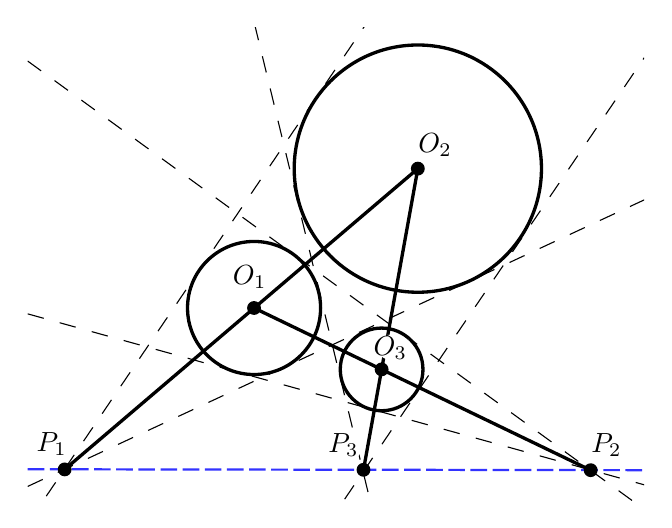
\begin{tikzpicture}[scale = 0.5]
    \clip(4.47,-5.82) rectangle (20.13,6.18);
    \draw [line width=1.2pt] (10.22,-0.94) circle (1.69cm);
    \draw [line width=1.2pt] (13.46,-2.5) circle (1.05cm);
    \draw [line width=1.2pt] (14.38,2.6) circle (3.14cm);
    \draw [line width=1.2pt] (5.41,-5.04)-- (14.38,2.6);
    \draw [line width=1.2pt] (14.38,2.6)-- (13,-5.05);
    \draw [line width=1.2pt] (10.22,-0.94)-- (18.77,-5.06);
    \draw [color = ttttff, dash pattern=on 6pt off 2pt, line width=0.8pt, domain=4.47:20.13] plot(\x,{(-67.19-0.02*\x)/13.36});
    \draw [dash pattern=on 6pt off 6pt,domain=4.47:20.13] plot(\x,{(-41.75--2.57*\x)/5.53});
    \draw [dash pattern=on 6pt off 6pt,domain=4.47:20.13] plot(\x,{(-44.52--5.05*\x)/3.42});
    \draw [dash pattern=on 6pt off 6pt,domain=4.47:20.13] plot(\x,{(-32.25--1.96*\x)/1.33});
    \draw [dash pattern=on 6pt off 6pt,domain=4.47:20.13] plot(\x,{(-27.15--2.31*\x)/-0.56});
    \draw [dash pattern=on 6pt off 6pt,domain=4.47:20.13] plot(\x,{(-40.25--3.41*\x)/-4.69});
    \draw [dash pattern=on 6pt off 6pt,domain=4.47:20.13] plot(\x,{(-0.84--1.55*\x)/-5.59});
    \begin{scriptsize}
        \normalsize
        \fill [color=black] (10.22,-0.94) circle (5pt);
        \draw[color=black] (10.11,-0.15) node[fill = white, rounded corners = 4pt, inner sep = 1pt] {$O_1$};
        \fill [color=black] (14.38,2.6) circle (5pt);
        \draw[color=black] (14.82,3.2) node {$O_2$};
        \fill [color=black] (13.46,-2.5) circle (5pt);
        \draw[color=black] (13.68,-1.95) node[fill = white, rounded corners = 8pt, inner sep = 0.5pt] {$O_3$};
        \fill [color=black] (5.41,-5.04) circle (5pt);
        \draw[color=black] (5.08,-4.4) node {$P_1$};
        \fill [color=black] (18.77,-5.06) circle (5pt);
        \draw[color=black] (19.17,-4.43) node {$P_2$};
        \fill [color=black] (13,-5.05) circle (5pt);
        \draw[color=black] (12.49,-4.43) node[fill = white, rounded corners = 4pt, inner sep = 1pt] {$P_3$};
    \end{scriptsize}
\end{tikzpicture}
        \caption{Teorema de Monge.}
    \end{figure}
    pero por definción, tenemos que
    \[
        \ratioCM{O_3}{O_1}{O_2}{P_3}{P_1}{P_2} = \dfrac{r_3}{r_1} \cdot \dfrac{r_1}{r_2} \cdot \dfrac{r_2}{r_3} = 1
    \]
    la conclusión es inmedianta. \qedhere
\end{proof}


\begin{section-theorem.tcb}{Monge D'Alembert}{monge-d-alembert-theorem}
    Sean $\Omega_1$, $\Omega_2$ y $\Omega_3$ tres circunferencias.
    El exsimilicentro de $\Omega_1$ y $\Omega_2$, el insimilicentro de $\Omega_2$ y $\Omega_3$, y el insimilicentro de $\Omega_3$ y $\Omega_1$ son colineales.
\end{section-theorem.tcb}
\begin{proof}
    Similar a la prueba del~\refTheorem{\ref{t:monge-theorem}}.
    Esta demostración se deja como ejercicio al lector.
\end{proof}

\begin{figure}[H]
    \centering
    \definecolor{ttttff}{rgb}{0.2,0.2,1}
%dash pattern=on 5pt off 2pt
%[fill = white, rounded corners = 4pt, inner sep = 1pt]
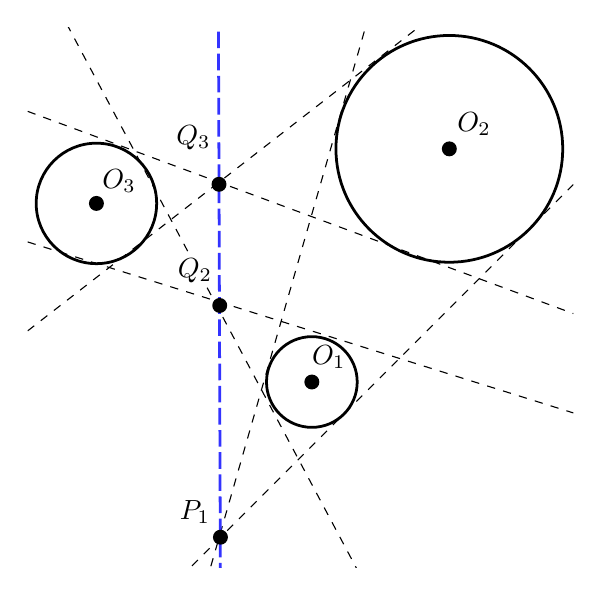
\begin{tikzpicture}[scale = 0.9]
    \clip(11.65,-5.82) rectangle (19.35,1.8);
    \draw [line width=1pt] (15.66,-3.2) circle (0.64cm);
    \draw [line width=1pt] (12.62,-0.68) circle (0.85cm);
    \draw [line width=1pt] (17.6,0.09) circle (1.6cm);
    \draw [line width=0.4pt,dash pattern=on 3pt off 3pt,domain=11.65:19.35] plot(\x,{(--18.33-1.39*\x)/0.74});
    \draw [line width=0.4pt,dash pattern=on 3pt off 3pt,domain=11.65:19.35] plot(\x,{(--3.64-0.47*\x)/1.5});
    \draw [line width=0.4pt,dash pattern=on 3pt off 3pt,domain=11.65:19.35] plot(\x,{(-7.06--0.53*\x)/-1.43});
    \draw [line width=0.4pt,dash pattern=on 3pt off 3pt,domain=11.65:19.35] plot(\x,{(--13.95-0.94*\x)/-1.21});
    \draw [line width=0.4pt,dash pattern=on 3pt off 3pt,domain=11.65:19.35] plot(\x,{(-34.39--1.74*\x)/1.74});
    \draw [line width=0.4pt,dash pattern=on 3pt off 3pt,domain=11.65:19.35] plot(\x,{(-37.68--2.37*\x)/0.68});
    \draw [line width=1pt, dash pattern = on 6pt off 2pt,color=ttttff] (14.34,2.37)-- (14.37,-6.12);
    \begin{scriptsize}
        \normalsize
        \fill [color=black] (15.66,-3.2) circle (3.0pt);
        \draw[color=black] (15.9,-2.85) node {$O_1$};
        \fill [color=black] (17.6,0.09) circle (3.0pt);
        \draw[color=black] (17.95,0.44) node {$O_2$};
        \fill [color=black] (12.62,-0.68) circle (3.0pt);
        \draw[color=black] (12.94,-0.36) node {$O_3$};
        \fill [color=black] (14.37,-5.39) circle (3.0pt);
        \draw[color=black] (14.01,-5.03) node[fill = white, rounded corners = 4pt, inner sep = 1pt] {$P_1$};
        \fill [color=black] (14.36,-2.12) circle (3.0pt);
        \draw[color=black] (14.01,-1.63) node[fill = white, rounded corners = 4pt, inner sep = 1pt] {$Q_2$};
        \fill [color=black] (14.35,-0.41) circle (3.0pt);
        \draw[color=black] (13.99,0.25) node[fill = white, rounded corners = 4pt, inner sep = 1pt] {$Q_3$};
    \end{scriptsize}
\end{tikzpicture}
    \caption{Teorema de Monge D'Alembert.}
\end{figure}



\subsubsection{Estrategias}
La homotecia en circunferencias resulta útil cuando:
\begin{itemize}
    \item Hay tangentes comunes.
    \item Hay circunferencias tangentes, interna o externamente.
    \item Hay cuerdas paralelas.
\end{itemize}

\subsubsection{Ejemplos}

\begin{section-example.tcb}{}{}
    Dos circunferencias iguales $C_1$ y $C_2$ son tangentes internamente a un circunferencia $C_3$ en dos puntos $A$ y $B$, respectivamente.
    Sea $C$ un punto en $C_3$.
    Si $D$ y $E$ son las intersecciones de $AC$ y $BC$ con $C_1$ y $C_2$, respectivamente, pruebe que $AB || DE$.
\end{section-example.tcb}
\begin{solution}
    Rápidamente nos damos cuenta de \homothety{A}{k}{C_1}{C_3} y \homothety{B}{k}{C_2}{C_3}.
    \begin{multicols}{2}
        \begin{figure}[H]
            \centering
            
%dash pattern=on 5pt off 2pt
%[fill = white, rounded corners = 4pt, inner sep = 1pt]
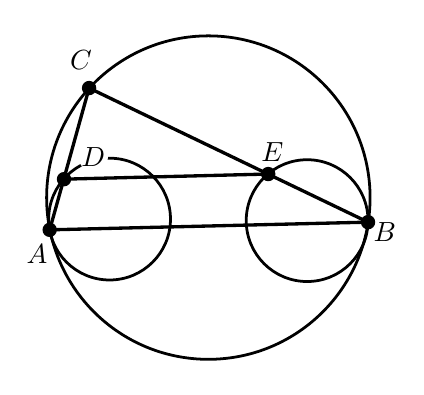
\begin{tikzpicture}[scale = 0.65]
    \clip(12.22,3.3) rectangle (19.42,9.93);
    \draw [line width=1pt] (13.82,6.19) circle (1.19cm);
    \draw [line width=1pt] (17.68,6.16) circle (1.19cm);
    \draw [line width=1pt] (15.75,6.61) circle (3.16cm);
    \draw [line width=1.2pt] (12.65,5.98)-- (18.87,6.13);
    \draw [line width=1.2pt] (18.87,6.13)-- (13.42,8.75);
    \draw [line width=1.2pt] (13.42,8.75)-- (12.65,5.98);
    \draw [line width=1.2pt] (12.93,6.97)-- (16.92,7.07);
    \begin{scriptsize}
        \normalsize
        \fill [color=black] (12.65,5.98) circle (4pt);
        \draw[color=black] (12.4,5.5) node[fill = white, rounded corners = 4pt, inner sep = 1pt] {$A$};
        \fill [color=black] (18.87,6.13) circle (4.0pt);
        \draw[color=black] (19.2,5.93) node {$B$};
        \fill [color=black] (12.93,6.97) circle (4.0pt);
        \draw[color=black] (13.5,7.4) node[fill = white, rounded corners = 4pt, inner sep = 1pt] {$D$};
        \fill [color=black] (16.92,7.07) circle (4.0pt);
        \draw[color=black] (17,7.5) node[fill = white, rounded corners = 4pt, inner sep = 1pt] {$E$};
        \fill [color=black] (13.42,8.75) circle (4.0pt);
        \draw[color=black] (13.26,9.3) node[fill = white, rounded corners = 4pt, inner sep = 1pt] {$C$};
    \end{scriptsize}
\end{tikzpicture}
        \end{figure}
        En la homotecia se tiene que $D \to C$ y $E \to C$, y cómo los radios son iguales la razón de homotecia es la misma, en este caso $k$, entonces
        \[
            \dfrac{AD}{AC} = \dfrac{BE}{BC} = k \quad \implies \quad AB || DE. \qedhere
        \]
    \end{multicols}
\end{solution}


\begin{section-example.tcb}{}{}
    Sea $ABCD$ un cuadrilátero convexo ex-inscrible\footnote{Existe una circunferencia tangente externamente a $AB$, $BC$, $CD$ y $DA$.} tal que $D$ es el más cercano a la circunferencia exinscrita.
    Sean $E$ y $F$ las intersecciones de $AB$ con $CD$ y $BC$ con $AD$, respectivamente, y sean $K$ y $L$ las intersecciones de las bisectrices de $\angle DAE$ con $DE$ y de $\angle DCF$ con $DF$, respectivamente.
    Demostrar que $AC$, $KL$ y la bisectriz del ángulo $\angle ADE$ concurren.
\end{section-example.tcb}
\begin{solution}
    Sea $\Gamma$ la circunferencia ex-inscrita a $ABCD$, y sean $\Gamma_1$ y $\Gamma_2$ los incírculos de $ADE$ y $CDF$, respectivamente.
    Llamemos $O$, $O_1$ y $O_2$ a los centros de $\Gamma$, $\Gamma_1$ y $\Gamma_2$ respectivamente.

    \begin{figure}[H]
        \centering
        
%dash pattern=on 5pt off 2pt
%[fill = white, rounded corners = 4pt, inner sep = 1pt]
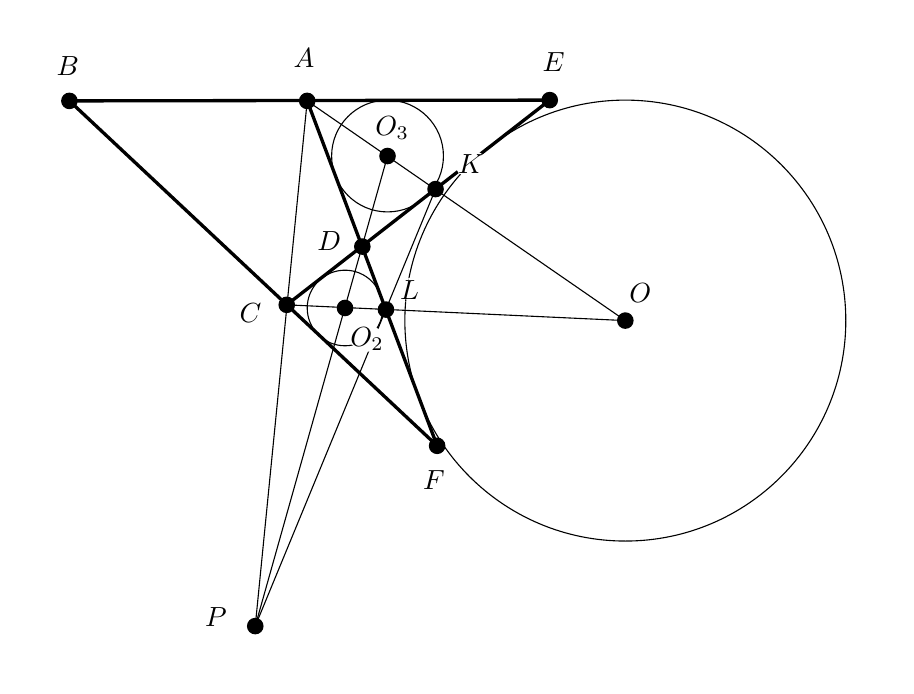
\begin{tikzpicture}[scale = 1]
    \clip(13.07,-0.17) rectangle (23.97,7.93);
    \draw(20.66,4.21) circle (2.8cm);
    \draw(17.1,4.37) circle (0.48cm);
    \draw(17.64,6.3) circle (0.71cm);
    \draw (16.62,7)-- (15.96,0.33);
    \draw (15.96,0.33)-- (17.64,6.3);
    \draw[line width=1.2pt] (18.27,2.62)-- (16.62,7);
    \draw[line width=1.2pt] (19.7,7.01)-- (16.36,4.41);
    \draw (20.66,4.21)-- (16.36,4.41);
    \draw (16.62,7)-- (20.66,4.21);
    \draw (15.96,0.33)-- (18.25,5.88);
    \draw[line width=1.2pt] (13.6,7)-- (19.7,7.01);
    \draw[line width=1.2pt] (13.6,7)-- (18.27,2.62);
    \begin{scriptsize}
        \normalsize
        \fill [color=black] (20.66,4.21) circle (3.0pt);
        \draw[color=black] (20.85,4.56) node {$O$};
        \fill [color=black] (13.6,7) circle (3.0pt);
        \draw[color=black] (13.58,7.44) node {$B$};
        \fill [color=black] (16.62,7) circle (3.0pt);
        \draw[color=black] (16.58,7.54) node {$A$};
        \fill [color=black] (18.27,2.62) circle (3.0pt);
        \draw[color=black] (18.23,2.19) node {$F$};
        \fill [color=black] (19.7,7.01) circle (3.0pt);
        \draw[color=black] (19.75,7.49) node {$E$};
        \fill [color=black] (16.36,4.41) circle (3.0pt);
        \draw[color=black] (15.9,4.3) node {$C$};
        \fill [color=black] (17.32,5.15) circle (3.0pt);
        \draw[color=black] (16.9,5.22) node {$D$};
        \fill [color=black] (17.62,4.35) circle (3.0pt);
        \draw[color=black] (17.92, 4.6) node[fill = white, rounded corners = 6pt, inner sep = 0.8pt] {$L$};
        \fill [color=black] (18.25,5.88) circle (3.0pt);
        \draw[color=black] (18.7,6.2) node[fill = white, rounded corners = 4pt, inner sep = 1pt] {$K$};
        \fill [color=black] (15.96,0.33) circle (3.0pt);
        \draw[color=black] (15.46,0.45) node {$P$};
        \fill [color=black] (17.1,4.37) circle (3pt);
        \draw[color=black] (17.38, 3.98) node[fill = white, rounded corners = 6pt, inner sep = 0.5pt] {$O_2$};
        \fill [color=black] (17.64,6.3) circle (3.0pt);
        \draw[color=black] (17.7,6.65) node[fill = white, rounded corners = 6pt, inner sep = 0.5pt] {$O_3$};
    \end{scriptsize}
\end{tikzpicture}
    \end{figure}

    Como $DE$ es la tangente común interna a $\Gamma$ y $\Gamma_1$, y además $AO$ es bisectriz, entonces $K$ es el centro de homotecia interno de $\Gamma$ y $\Gamma_1$.
    De manera análoga $L$ es el centro de similitud interno entre $\Gamma$ y $\Gamma_2$.
    Pero $A$ y $C$ son los centro de homotecia externa de $\Gamma$ con $\Gamma_1$ y $\Gamma$ con $\Gamma_2$, respectivamente, entonces por el~\refTheorem{\ref{t:monge-d-alembert-theorem}} $AC$ y $KL$ deben cortarse en el centro de homotecia externo de $\Gamma_1$ y $\Gamma_2$, y así la recta $O_1 O_2$, que es la bisectriz de $\angle ADE$, debe pasar por dicho punto.
\end{solution}




\subsection{Agregados culturales y preguntas}

\begin{itemize}
    \item La palabra \textbf{homotecia} deriva del griego \textit{homo} = semejante, y del \textit{tithénai} = colocar, disponer.
    \item El triángulo medial es el que se forma con los puntos medios de los lados de un triángulo dado.
    \item La composición de dos homotecias se logra aplicando una homotecia con un centro dado, y a esa transformación se le aplica otra homotecia con otro centro dado.
    El resultado vendría siendo algo como una homotecia de la homotecia inicial.
    \item Existe una transformación llamada \textbf{semejanza espiral} o \textbf{rotohomotecia}.
    La cual es una composición de una homotecia y una rotación respecto a un centro dado.
    Esta transformación es muy útil en la resolución de problemas de mayor dificultad.
\end{itemize}



\subsection{Ejercicios y Problemas}

Sección de ejercicios y problemas para el autoestudio.

\begin{section-exercise}
    Da un triángulo \theTriangle{ABC} y punto $O$ fuera de él, construye con regla y compas un triángulo \theTriangle{XYZ} tal que \homothety{O}{2}{\theTriangle{ABC}}{\theTriangle{XYZ}}.
\end{section-exercise}


\begin{section-problem}
    Dado el triángulo \theTriangle{ABC} y su circuncírculo $\Omega$, demostrar que el triángulo medial $A' B' C'$ es homotético al triángulo \theTriangle{ABC}.
    Encontrar el centro de homotecia y la razón de homotecia.
\end{section-problem}

\begin{section-problem}
    Demostar que si dos circunferencias son tangentes internamente en un punto $A$ y si una secante común interseca a las circunferencias en $B'$, $B$, $C$ y $C'$, entonces $\angle B' AC = \angle BAC'$.
\end{section-problem}

\begin{section-problem}
    El \theTriangle{ABC} tiene inscrita una circunferencia.
    Supongamos que $M$ es el punto de tangencia de la circunferencia con el lado $AC$, $MK$ es el diámetro.
    La recta $BK$ corta $AC$ en el punto $N$.
    Demostrar que $AM = NC$
\end{section-problem}

\begin{section-problem}
    El incírculo de \theTriangle{ABC} tiene centro $I$ y toca a $BC$ en $E$.
    $AD$ es una altura de \theTriangle{ABC}, $M$ es el punto medio $AD$.
    Sea $I_A$ el A-excentro de \theTriangle{ABC}.
    Demostrar que $M$, $E$ e $I_A$ con colienales.
\end{section-problem}

\begin{section-problem}
    Sea $\Omega$ y $\Gamma$ dos círculos tangentes en $D$, de forma que $\Gamma$ yace en el interior de $\Omega$.
    Se traza una cuerda de $AB$ en $\Omega$ de modo que $AB$ es tangente a $\Gamma$ en $C$.
    Probar que $DC$ bisecta al arco $\wideparen{AB}$ que no contiene a $AD$.
\end{section-problem}